\section{Results}
\label{sec:results}

\subsection{Placeholder plant}
Table~\ref{tab:results1} and Fig.~\ref{fig:energyrob} summarise the robust retraining.
On the nominal model the PID with gravity feed-forward is the most efficient controller
(68.6\,kJ per move, 1.0\,\% misses), and every SAC policy uses more energy
(100.8--173.6\,kJ). The PID, however, fails as soon as the model is wrong: with a payload step
of $\times1.2$ it misses on 100\,\% of the moves, with the angle-dependent torque limit on 45\,\%
and with the boom-only mass on 100\,\% (Fig.~\ref{fig:robbars}). Adding integral action reduces
the payload misses to 37\,\% at 97.7\,kJ.
Domain-randomised SAC keeps the payload misses at 3.0--8.0\,\% and the torque-limit misses at
1.7--6.0\,\%. SAC with $w=0.3$ uses about the energy of the PID with integral action
(100.8 vs 97.7\,kJ) with 3.0\,\% instead of 37\,\% payload misses, and residual SAC with
$w=0.1$ is the only controller without misses on out-of-range targets.
Fig.~\ref{fig:payload} shows a move with a payload step for the PID and for SAC.
% TODO: one sentence on what Fig 3 shows (check the figure; do not guess).
The boom-only mass ($\times0.42$) remains the hardest case for most controllers
(16--67\,\% misses); only residual SAC with $w=0$ handles it (1.3\,\%).
On the placeholder plant, SAC therefore buys robustness to model error at an energy cost.

\begin{table*}[t]
\caption{Placeholder plant: robust retraining, 100 unseen scenarios (SAC: mean of 3 seeds)}
\label{tab:results1}
\centering
% Source: rl/08b_eval_n10.csv. Seeds: mean of means, worst of maxima, mean of shares.
\begin{tabular}{lrrrrrl}
\hline
Controller & Mean & Worst & Energy & $>$20\,cm & out100 $>$20\,cm & Worst variant $>$20\,cm \\
 & [cm] & [cm] & [kJ] & [\%] & [\%] & [\%] \\
\hline
plain w=0.0 & 7.0 & 39.8 & 173.6 & 7.7 & 9.7 & 18.7 (m\_x0.42) \\
plain w=0.1 & 5.5 & 40.0 & 127.9 & 3.7 & 10.0 & 16.3 (m\_x0.42) \\
plain w=0.3 & 6.1 & 55.2 & 100.8 & 1.3 & 7.3 & 66.7 (m\_x0.42) \\
residual w=0.0 & 4.9 & 29.1 & 150.8 & 4.3 & 18.0 & 5.3 (tau\_d) \\
residual w=0.1 & 5.2 & 23.0 & 124.7 & 2.3 & 0.0 & 26.0 (m\_x0.42) \\
residual w=0.3 & 6.4 & 26.1 & 103.1 & 1.7 & 9.7 & 63.3 (m\_x0.42) \\
pid & 7.1 & 21.4 & 68.6 & 1.0 & 18.0 & 100.0 (m\_x0.42) \\
pid\_ki & 8.5 & 21.6 & 97.7 & 1.0 & 14.0 & 99.0 (m\_x0.42) \\
\hline
\end{tabular}

\end{table*}

\begin{figure}[t]
\centering
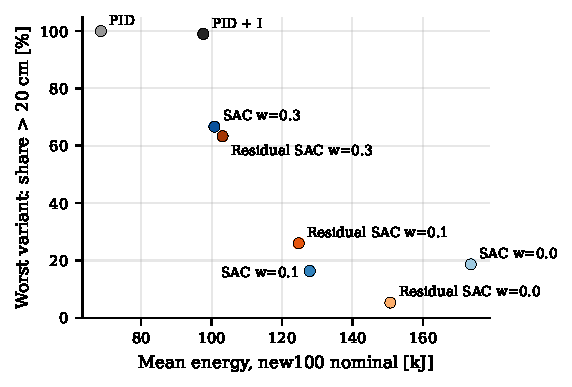
\includegraphics[width=\columnwidth]{figs/fig1_energy_vs_robustness.pdf}
\caption{Placeholder plant: nominal energy against misses under model error.}
\label{fig:energyrob}
\end{figure}

\begin{figure}[t]
\centering
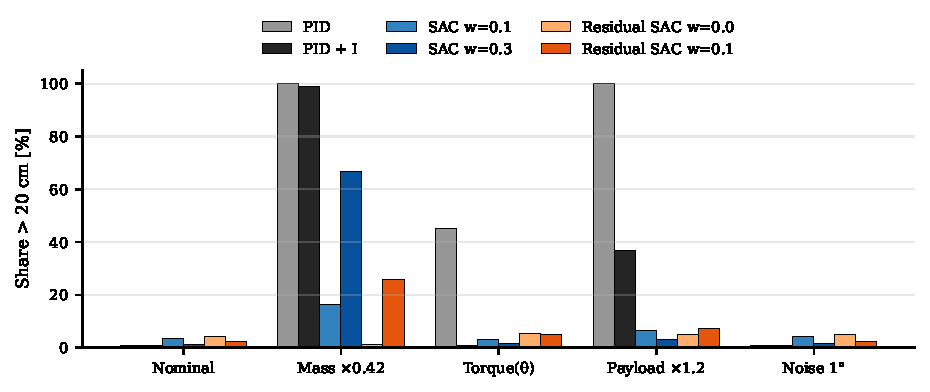
\includegraphics[width=\columnwidth]{figs/fig2_robustness_bars.pdf}
\caption{Placeholder plant: share of moves over 20\,cm for each robustness case.}
\label{fig:robbars}
\end{figure}

\begin{figure}[t]
\centering
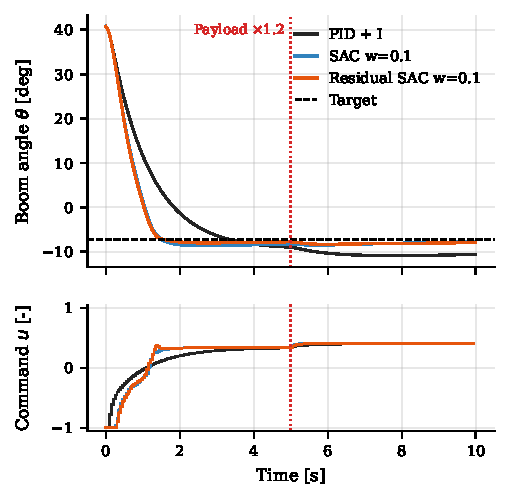
\includegraphics[width=\columnwidth]{figs/fig3_payload_trajectory.pdf}
\caption{Placeholder plant: boom angle after a payload step ($\times1.2$), PID and SAC.}
\label{fig:payload}
\end{figure}
% TODO: check each caption against what the figure actually shows.

\subsection{Real-parameter plant}
Table~\ref{tab:results2} gives the results on the real-parameter plant over all 72 test rows
of 100 unseen moves. The PID with the tip-mass estimator misses on none of the 7200 moves at any
of its three operating points, with 159.1--180.3\,kJ per move, 20.0--36.0\,\% above the energy
floor. The robustness that SAC added on the placeholder plant is thus already provided by the
mass estimate.
Neither SAC structure improves on the PID in energy or in accuracy.
Residual SAC is as fast as the balanced PID (1.46\,s to come within 20\,cm) but uses 18.5\,kJ
more per move and misses on 3.3\,\% of the moves; its four broken rows are all low-inertia
cases with a dumped bucket. Plain SAC misses on 16.2\,\% and breaks every row.
Training with sensor noise lowers the energy of residual SAC to 173.7\,kJ, still above all three
PID points, but raises its misses to 24.6\,\%, and to 23.3\,\% even without sensor noise: the
policy saves energy by not completing moves. The seeds differ widely (residual SAC 1.6--4.7\,\%
misses, plain SAC 8.3--22.6\,\%).

\begin{table}[t]
\caption{Real-parameter plant: 72 test rows $\times$ 100 unseen moves (SAC: $w=0.1$, mean of 3 seeds)}
\label{tab:results2}
\centering
\footnotesize
\setlength{\tabcolsep}{3pt}
\begin{tabular}{lrrrrr}
\hline
Controller & Miss & Rows & $E$ & Gap & $t_{20}$ \\
 & [\%] & brk/deg & [kJ] & [\%] & [s] \\
\hline
PID fast & 0.00 & 0/0 & 180.3 & 36.0 & 1.19 \\
PID balanced & 0.00 & 0/0 & 167.5 & 26.4 & 1.46 \\
PID economical & 0.00 & 0/0 & 159.1 & 20.0 & 1.99 \\
Residual SAC & 3.31 & 4/68 & 186.1 & 40.4 & 1.46 \\
Plain SAC & 16.22 & 72/0 & 186.2 & 40.5 & 1.73 \\
Residual SAC, noise & 24.56 & 72/0 & 173.7 & 31.1 & 2.49 \\
\hline
\end{tabular}
\end{table}
% Source: rl/12_eval.md section 1. brk = rows over 5 % misses, deg = 1-5 %.

\subsection{Where the remaining energy goes}
Sensor noise is the main driver of the remaining gap. Without sensor noise the economical PID is
10.7\,\% above the floor; with $1^\circ$ noise it is 37.0\,\%, and the same growth appears for every
controller. Splitting the excess of the balanced PID by the angle each step covers, overshoot
accounts for 12.5\,kJ, repeated passes (oscillation) for 16.8\,kJ and the direct path for
5.6\,kJ per move. Most of the remaining energy is therefore spent on overshoot and oscillation
that noise excites, not on the direct move.
% Source: rl/12_eval.md sections 1-2. Lab 12a speed filter: gap 24.0 -> 23.8 % (tuning set).
